%**************************************************************
% CAPITOLO 1
%**************************************************************
\chapter{The White Dog s.r.l.}
\label{cap:thewhitedog}

\section{Chi è The White Dog s.r.l.}

The White Dog s.r.l. è una realtà aziendale nata nel 2008 con sede a Torreglia, in provincia di Padova. Essa è stata fondata dal signor Stefano Mocellini, fondatore e CEO di Diana Corp.\footnote[1]{\url{http://www.dianacorp.com/}}, con la volontà di creare un \textit{team} di lavoro focalizzato sulla ricerca e sviluppo per quest'ultima. \\
The White Dog s.r.l. coordina e gestisce società tutte affini al settore \textit{e-commerce}, come Diana Corp. e LiveStory\footnote[2]{\url{http://www.livestory.nyc/}}. L'azienda possiede un reparto di ricerca e sviluppo denominato R\&D, il quale esplora nuove tecnologie da applicare poi alle società figlie nel caso di esito positivo o facendo nascere nuovi progetti separati.

\label{The White Dog s.r.l.}
\begin{figure}[ht]
	\begin{center}
		
\includegraphics[scale=1]{twd_logo}
		\caption{Logo dell'azienda The White Dog s.r.l.}
	\end{center}
\end{figure}
\FloatBarrier

\section{Prodotti e servizi}

L'azienda svolge principalmente due attività: la prima legata al servizio di supporto tecnologico offerto a Diana Corp., la seconda legata alla gestione e sviluppo del prodotto Live Story.

\subsection{Servizio di supporto tecnologico}

Il principale servizio che l'azienda offre a Diana Corp. è la ricerca e lo sviluppo di nuove tecnologie da applicare nell'ambito del \textit{fashion e-commerce}. \\
\textit{E-commerce} è l'acronimo di \textit{Electronic Commerce} e consiste nella presentazione, vendita e gestione di prodotti utilizzando strumenti elettronici, in particolare siti internet dedicati. Avere un sito \textit{e-commerce}, o implementare il pagamento degli acquisti sul proprio sito web, offre la possibilità ad una azienda di estendere a livello globale i propri potenziali clienti, espandendo così il proprio \textit{business}. La sicurezza delle operazioni di acquisto viene garantita tramite l'utilizzo di server sicuri, caratterizzati dall'indirizzo HTTPS, un apposito protocollo che crittografa i dati sensibili dei clienti contenuti nell'ordine di acquisto allo scopo di tutelare il consumatore.

\label{E-commerce}
\begin{figure}[ht]
	\begin{center}
		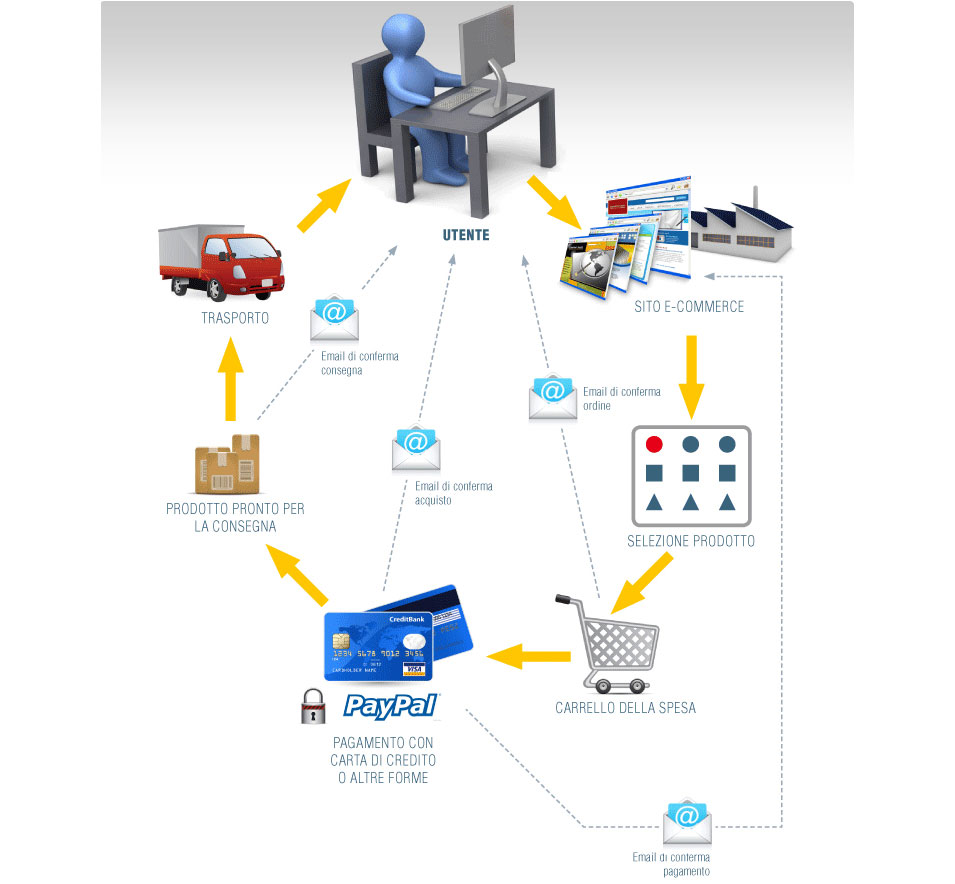
\includegraphics[scale=0.4]{ecommerce}
		\caption{Processo d'acquisto tramite \textit{e-commerce}. Immagine tratta dal sito dell'azienda LEVERPLAN: \url{http://www.leverplan.com/it/agenzia_web_agency/ecommerce.aspx}}
	\end{center}
\end{figure}
\FloatBarrier

Diana Corp., principale cliente di The White Dog s.r.l. e sua azienda d'origine, propone ai sui clienti un portale \textit{e-commerce} che comprende la gestione dei prodotti, del design, dell'infrastruttura e della manutenzione. Inoltre, il pacchetto può essere arricchito sia con soluzioni di marketing, come \textit{newsletter} o campagne, sia con la gestione delle spedizioni, ospitando i prodotti nel magazzino dell'azienda. Alcune delle principali piattaforme sviluppate da Diana Corp. sono ad esempio The Blonde Salad\footnote[3]{\url{http://www.theblondesalad.com/it/}} e Pryma\footnote[4]{\url{http://www.pryma.com/it_it/}}. \\
The White Dog s.r.l. svolge un'attività di \textit{testing}\ped{\hyperlink{test}{G}} dei nuovi strumenti presenti nel mercato da applicare agli \textit{e-commerce} di Diana Corp., li valuta attentamente in termini di prestazioni e costi, per poi renderli disponibili agli sviluppatori di quest'ultima attraverso consulenze. \\
The White Dog s.r.l., inoltre, interviene direttamente nel codice dei servizi Diana Corp. se a quest'ultima vengono commissionate nuove \textit{features} o applicazioni che, per tempistiche o competenze, non è in grado da sola di sviluppare. \\
Infine, offre consulenza a Diana Corp. per l'utilizzo delle seguenti piattaforme di \textit{management}:

\begin{itemize}
	\item \textbf{SAP:} sistema informativo per la gestione di tutti i processi aziendali. SAP supporta il sistema di gestione ERP, acronimo di \textit{Enterprise Resource Planning}, il quale, come è visibile nella \hyperlink{f1.3}{figura 1.3}, integra e gestisce tutti i processi di \textit{business} rilevanti di un'azienda: vendite, acquisti, gestione magazzino, contabilità, produzione e salvataggio dei dati. ERP fornisce una visione dei processi di business, spesso in tempo reale, utilizzando \textit{database} comunemente gestiti da un \textit{database management system}. Esso traccia risorse come contanti, materie prime, capacità di produzione e lo stato degli impegni lavorativi come ordini, ordini d'acquisto e libro paga. Facilita il flusso di informazioni tra tutte le funzioni aziendali e gestisce le connessioni agli \textit{stakeholder}\hyperlink{sh}{\ped{G}} esterni. \\
	Nel caso dell'azienda Diana Corp. il sistema ERP contiene le informazioni riguardanti i prodotti e lo stato del magazzino. Alcune delle informazioni, come la descrizione e la disponibilità del prodotto, vengono sincronizzate con la piattaforma di vendita. \\
	Al termine di ogni ordine, il portale \textit{e-commerce} notifica il sistema ERP le seguenti operazioni:
	\begin{itemize}
		\item Contabilizzazione del pagamento;
		\item Aggiornamento dello stato del magazzino, decrementando la quantità disponibile della merce appena ordinata;
		\item Generazione della fattura.
	\end{itemize}
	
	\item \textbf{Magento:} è una piattaforma \textit{e-commerce} \textit{open source} che offre la possibilità di avviare una attività online di commercio elettronico con ampia flessibilità sia nella grafica, sia nelle funzionalità che nei contenuti. \\
	L’interfaccia di amministrazione fornisce strumenti di marketing, SEO e gestione del catalogo, in modo da offrire ai commercianti la possibilità di creare siti a misura delle proprie esigenze di business. Progettato per essere completamente scalabile e per essere ripristinato facilmente.
	
	\item \textbf{WordPress:} è una piattaforma software di \textit{personal publishing} e \textit{content management system}\ped{\hyperlink{cms}{G}}, ovvero un programma che consente la creazione e distribuzione di un sito internet formato da contenuti testuali o multimediali, facilmente gestibili ed aggiornabili in maniera dinamica.	
\end{itemize}
 
\label{ERP}
\begin{figure}[ht]
	\begin{center}
		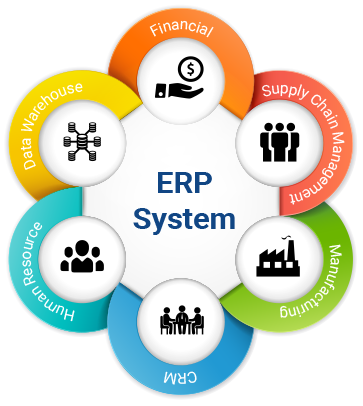
\includegraphics[scale=0.5]{erp}
		\hypertarget{f1.3}{\caption{Ambiti aziendali gestiti dal sistema ERP. Immagine tratta dal sito della compagnia di sviluppo software KNOWART: \url{http://www.knowarth.com/enterprise-resource-planning/}}}
	\end{center}
\end{figure}
\FloatBarrier

\subsection{Il prodotto Live Story}

Live Story è un \textit{social management system}\ped{\hyperlink{sms}{G}} che gestisce contenuti \textit{social} e li rende acquistabili. Il \textit{concept} di Live Story è nato nel reparto R\&D di The White Dog s.r.l., \textit{concept} che è diventato poi azienda nel 2015 con sede a New York. \\
Live Story è una piattaforma, resa disponibile alle aziende di moda, che colleziona foto degli utenti dei \textit{social network}, come \textit{Facebook}, \textit{Instagram} e \textit{Twitter}, marcate da particolari \textit{hashtag}. Tali \textit{hashtag} rappresentano i vari prodotti dell'azienda che utilizza il servizio Live Story, la quale invita i propri clienti ad utilizzarli all'interno dei \textit{social media}. Il sistema accoppia la foto marcata ad un particolare prodotto presente nel catalogo aziendale e genera automaticamente le richieste di permesso di sfruttamento della foto, inviandola all'utente interessato. Se l'utente approva e il moderatore aziendale ritiene conforme la foto, l'azienda può utilizzare il contenuto nel proprio sito o \textit{e-commerce}. \\
Una volta approvati, i contenuti possono comporre un \textit{wall}, ovvero un pannello dei prodotti visibile in una pagina web. Vi sono due tipi di \textit{wall} che Live Story permette di comporre:

\begin{itemize}
	\item \textbf{Mood:} \textit{wall} creati con contenuti e foto scelti dall'azienda. In questo caso non vi è nessuna interazione con gli utenti dei \textit{social network}, ma solo una creazione più rapida dei contenuti visualizzabili nell'\textit{e-commerce};
	\item \textbf{Feed:} \textit{wall} creati automaticamente tramite i contenuti marcati dagli \textit{hashtag} aziendali presenti nei \textit{social network}.
\end{itemize}

Ogni \textit{wall} è personalizzabile e ogni \textit{brand} può definire il proprio stile tramite fogli CSS.

\label{Wall}
\begin{figure}[ht]
	\begin{center}
		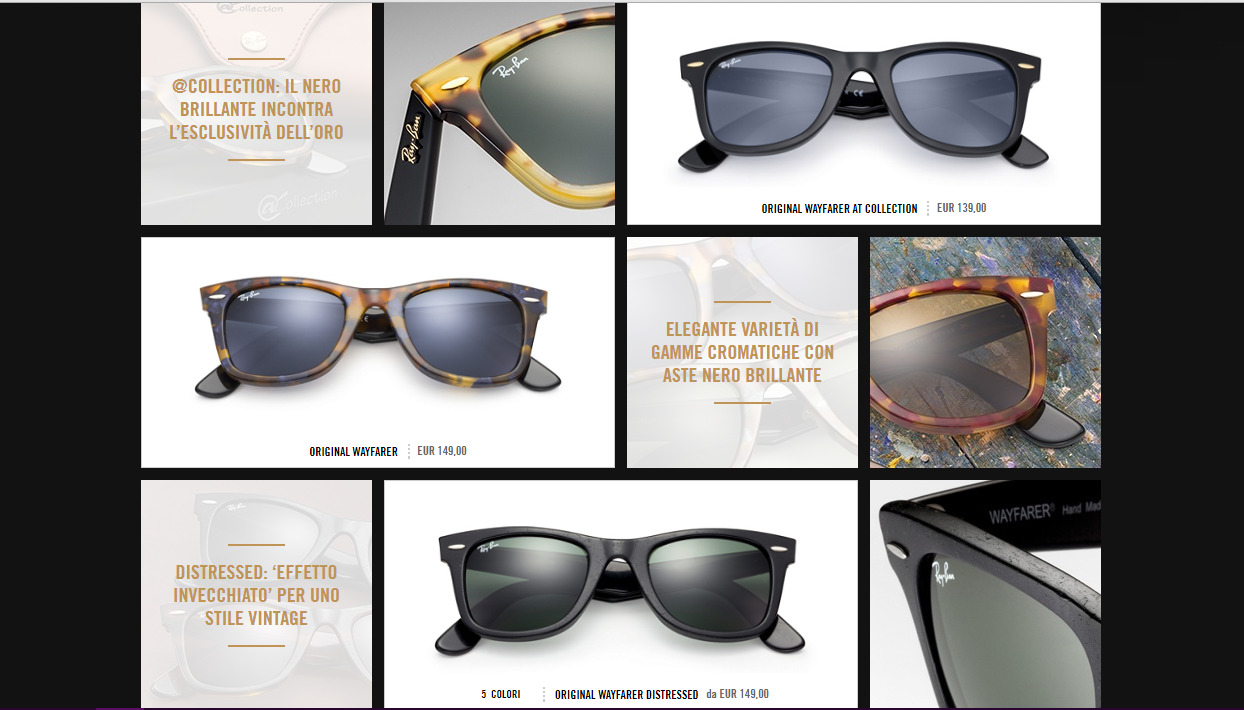
\includegraphics[scale=0.39]{wall}
		\caption{\textit{Wall mood} creato tramite \textit{Live Story} per l'\textit{e-commerce} di una nota marca di occhiali: \url{http://www.ray-ban.com/italy}}
	\end{center}
\end{figure}
\FloatBarrier

\section{Processi interni}

Lo sviluppo del software a The White Dog s.r.l. segue una metodologia tipicamente Agile\footnote[5]{\url{http://agilemanifesto.org/}}. \\ 
La Metodologia Agile si riferisce ad un insieme di metodi di sviluppo software fondati su principi comuni, direttamente o indirettamente derivati dai principi del \textit{Manifesto per lo Sviluppo Agile di Software}: 

\begin{itemize}
	\item \textbf{Gli individui e le interazioni} più che i processi e gli strumenti;
	\item \textbf{Il software funzionante} più che la documentazione esaustiva;
	\item \textbf{La collaborazione col cliente} più che la negoziazione dei contratti;
	\item \textbf{Rispondere al cambiamento} più che seguire un piano.
\end{itemize}

I metodi agili si contrappongono al modello a cascata e ad altri processi software tradizionali, proponendo un approccio meno strutturato e focalizzato sull'obbiettivo di consegnare al cliente, in tempi brevi e frequentemente, software funzionante e di qualità. Fra le pratiche promosse dai metodi agili ci sono la formazione di team di sviluppo piccoli, cross-funzionali e auto-organizzati, lo sviluppo iterativo e incrementale, la pianificazione adattiva e il coinvolgimento diretto e continuo del cliente nel processo di sviluppo. 

\label{Metodologia Agile}
\begin{figure}[ht]
	\begin{center}
		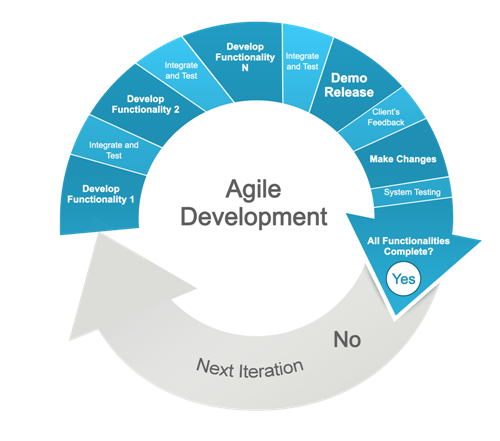
\includegraphics[scale=2.25]{agile_development}
		\caption{Ciclo di sviluppo della Metodologia Agile. Immagine tratta dal sito informativo Quora: \url{https://www.quora.com/}}
	\end{center}
\end{figure}
\FloatBarrier

L'azienda The White Dog s.r.l. è composta da un \textit{team} di sviluppo formato da sole tre persone, le quali possiedono competenze sia software, sia decisionali che di controllo della qualità. Questo permette all'azienda di essere molto agile sia nello sviluppo che nel rilascio del software. \\ 
Essa dà molta importanza agli individui presenti e all'interazione tra di loro, eliminando completamente la gerarchia lavorativa classica e impegnandosi molto per mantenere un ambiente lavorativo di reciproco rispetto paritario. \\
La collaborazione col cliente avviene in maniera assidua e giornaliera tramite riunioni nell'ufficio R\&D o con trasferte. Se entrambe le soluzioni non sono attuabili, vengono optate sessioni di video conferenze. Questa pratica è agevolata dal fatto che per volontà del fondatore, The White Dog s.r.l. ha sede all'interno dello stesso stabilimento di Diana Corp., suo principale cliente. \\
Infine la natura dell'azienda la obbliga a rispondere al cambiamento in maniera molto veloce e repentina, dovendo pianificare così molti cicli di \textit{refactoring}\ped{\hyperlink{ref}{G}} per lo sviluppo software. \\ \\

Le tre principali metodologie di sviluppo, derivanti da quella Agile, che l'azienda adotta sono:

\subsubsection{DevOps}

Metodologia di sviluppo software che punta alla comunicazione, collaborazione e integrazione tra gli sviluppatori e addetti alle \textit{operations}\ped{\hyperlink{ops}{G}} dell'\textit{information technology}. DevOps vuole rispondere all'interdipendenza tra sviluppo software e IT \textit{operations}\ped{\hyperlink{ops}{G}}, puntando ad aiutare un'organizzazione a sviluppare in modo più rapido ed efficiente prodotti e servizi. \\
L'integrazione \textit{DevOps} ha come obiettivo il rilascio del prodotto, il collaudo del software, l'evoluzione e il mantenimento in modo tale da aumentare affidabilità e sicurezza e rendere più veloci i cicli di sviluppo e rilascio. 

\label{DevOps}
\begin{figure}[ht]
	\begin{center}
		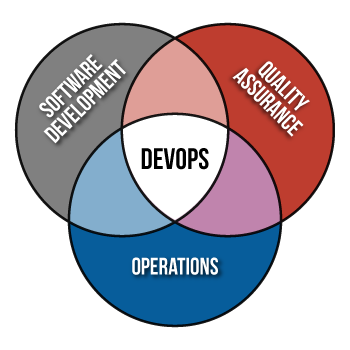
\includegraphics[scale=0.5]{devops-diagram}
		\caption{Competenze necessarie alla metodologia di sviluppo DevOps. Immagine tratta dal sito dell'organizzazione RTTS: \url{http://www.rttsweb.com/services/strategy/software-process-assessment}}
	\end{center}
\end{figure}
\FloatBarrier

In The White Dog s.r.l. questo principio è concretizzato dal fatto che ogni membro possiede sia le competenze di sviluppo, sia amministrative che di controllo della qualità, migliorando così di molto l'efficienza e l'agilità nello sviluppo del software. \\
Questa metodologia aiuta e migliora anche i continui rilasci che l'azienda giornalmente è costretta a fare per migliorare i servizi di Diana Corp. o per aumentarne le potenzialità con nuove tecnologie.

\subsubsection{Extreme Programming}

Metodologia di sviluppo software che enfatizza la scrittura di codice di qualità e la rapidità di risposta ai cambiamenti di requisiti. Prescrive lo sviluppo iterativo e incrementale, soprattutto in brevi cicli di sviluppo. Suggerisce inoltre l'uso sistematico di \textit{unit testing}\ped{\hyperlink{ut}{G}} e \textit{refactoring}\ped{\hyperlink{ref}{G}}, vietando ai programmatori di sviluppare codice non strettamente necessario. Sostiene la chiarezza e la semplicità del codice, preferisce strutture gestionali non gerarchiche e dà molta importanza alla comunicazione diretta e frequente fra sviluppatori e cliente e fra gli sviluppatori stessi. 

\label{Extreme Programming}
\begin{figure}[ht]
	\begin{center}
		
\includegraphics[scale=0.11]{extremeprogramming}
		\caption{Ciclo di sviluppo software Extreme Programming. Immagine tratta dalla pagina Wikipedia dedicata all'\textit{extreme programming}: \url{https://en.wikipedia.org/wiki/Extreme_programming}}
	\end{center}
\end{figure}
\FloatBarrier

Il \textit{team} di sviluppo di The White Dog s.r.l. fa ampio utilizzo di questa metodologia, spingendo molto sulla semplicità del codice prodotto, che andrà a migliorare e ampliare i servizi \textit{e-commerce} di Diana Corp. e Live Story e che quindi dovrà poi essere compreso dai loro sviluppatori. \\
Prevede continui cicli di \textit{refactoring}\ped{\hyperlink{ref}{G}} per adattarsi alla volubilità del cliente finale e di \textit{unit testing}\ped{\hyperlink{ut}{G}} per garantirgli codice funzionante e di qualità.

\subsubsection{Scrum}

\textit{Framework}\ped{\hyperlink{fw}{G}} agile di sviluppo software, iterativo ed incrementale, concepito per gestire progetti e prodotti software. Esso enfatizza tutti gli aspetti di gestione di progetto legati a contesti in cui è difficile pianificare in anticipo. Vengono utilizzati meccanismi propri di un processo di controllo empirico, in cui i cicli di \textit{feedback}, che ne costituiscono le tecniche di \textit{management} fondamentali, risultano in opposizione alla gestione basata sul concetto tradizionale di \textit{command-and-control}\ped{\hyperlink{cac}{G}}. Il suo approccio alla pianificazione e gestione dei progetti è quello di portare l'autorità decisionale al livello di proprietà e certezze operative.

\label{Scrum board}
\begin{figure}[ht]
	\begin{center}
		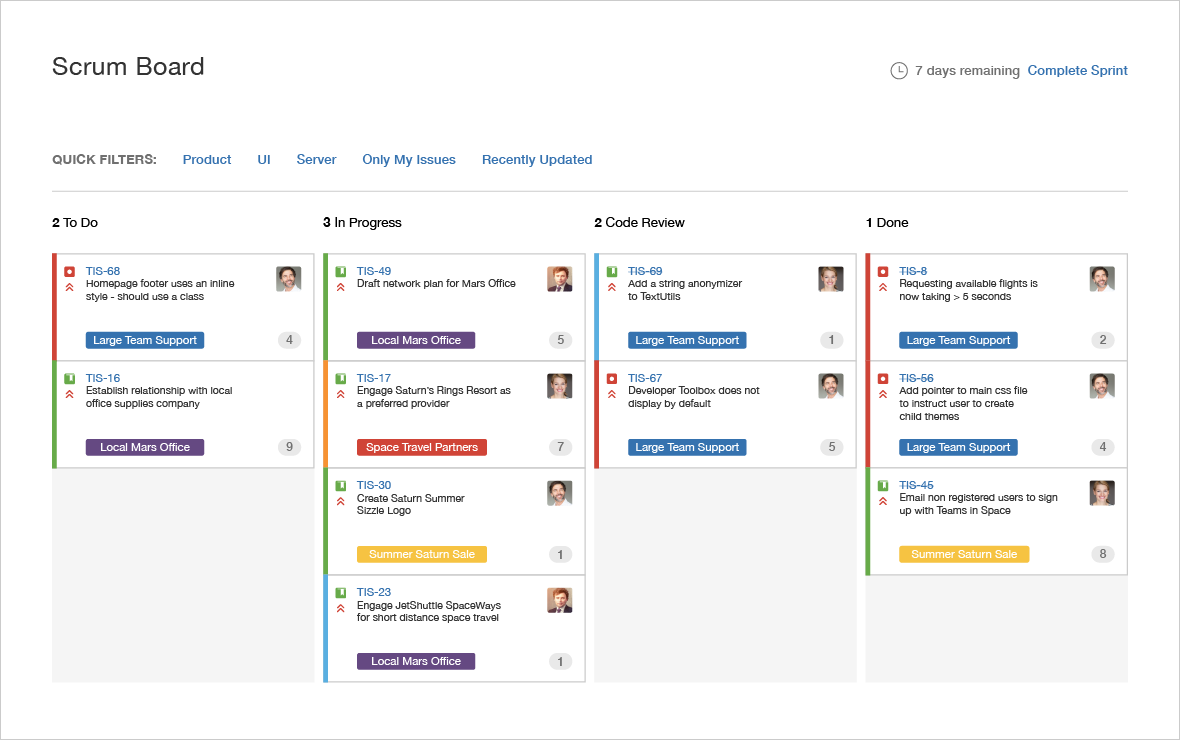
\includegraphics[scale=0.30]{scrumboard}
		\caption{Esempio di \textit{scrum board} all'interno del servizio Jira}
	\end{center}
\end{figure}
\FloatBarrier

Data la forte difficoltà aziendale a pianificare in anticipo lo sviluppo software, causata dalla continua richiesta di modifiche e nuove funzionalità dei servizi \textit{e-commerce} che ha in gestione, l'azienda fa ampio utilizzo di questa metodologia di pianificazione del lavoro utilizzando strumenti di \textit{project management} come Wrike\footnote[6]{\url{https://www.wrike.com/it/it/}} e Jira\footnote[7]{\url{https://www.atlassian.com/software/jira}}. I due software supportano il principio \textit{Scrum} fornendo all'utente una \textit{Scrum board}: tavola virtuale nella quale è possibile visualizzare il flusso di lavoro suddiviso in sezioni. Ad ogni sezione sono assegnati uno o più sviluppatori che annotano l'avanzamento del lavoro, i \textit{bug} e i problemi riscontrati. 

\section{Strumenti e tecnologie}

\subsection{Ambienti di sviluppo}

Il sistema operativo adottato dall'azienda è Mac OS X installato su macchine iMac. \\
L'ambiente di sviluppo predefinito è Eclipse\footnote[8]{\url{https://eclipse.org/}}, ma, data la natura aziendale, varia molto spesso in base al prodotto in fase di sviluppo, che può cambiare in maniera repentina. 

\subsection{Gestione dei progetti}

I due principali strumenti utilizzati da The White Dog s.r.l. per il \textit{project management} e l'\textit{issue tracking}\ped{\hyperlink{it}{G}} sono rispettivamente Wrike e Jira.\\
Wrike, sviluppato dall'omonima casa, è uno strumento per la collaborazione e il \textit{project management}. Permette ai suoi utenti di modificare progetti, classificare le attività per importanza, tenere traccia dei programmi e collaborare con altri utenti dello stesso gruppo. \\
Jira, prodotto dall'azienda Atlassian, è un software di \textit{bug tracking}\ped{\hyperlink{bg}{G}}, \textit{issue tracking}\ped{\hyperlink{it}{G}} e \textit{project management}. Esso permette di tenere traccia delle azioni e dei problemi degli utenti, di distribuire i compiti all'interno del \textit{team}, discutere del lavoro in atto con una visibilità completa e migliorare le prestazioni della squadra visualizzando dati in tempo reale.

\subsection{Versionamento}

Il principale software di controllo di versione distribuito utilizzato dall'azienda è Git\footnote[9]{\url{https://git-scm.com/}}. Git supporta lo sviluppo non lineare con diramazione e fusioni rapide e continue e comprende strumenti specifici per visualizzare e navigare una cronologia di sviluppo. Permette ad ogni sviluppatore una copia locale dell'intera cronologia di sviluppo e le modifiche vengono importate da un \textit{repository}\ped{\hyperlink{rep}{G}} ad un altro. I \textit{repository}\ped{\hyperlink{rep}{G}} possono essere pubblicati facilmente tramite protocolli HTTP, FTP, SSH, RSYNC o uno speciale protocollo git.

\subsection{Strumenti di automazione}

The White Dog s.r.l. fa ampio utilizzo di strumenti si automazione per facilitare il \textit{deployment}\ped{\hyperlink{dep}{G}} del software prodotto. \\
Il principale strumento utilizzato dall'azienda è Docker\footnote[10]{\url{https://www.docker.com/}}. Docker è un progetto \textit{open-source} che automatizza il \textit{deployment}\ped{\hyperlink{dep}{G}} delle applicazioni all'interno di \textit{container software}\ped{\hyperlink{cs}{G}}, fornendo un'astrazione addizionale grazie alla virtualizzazione a livello di sistema operativo Linux. Docker utilizza le funzionalità di isolamento delle risorse del kernel Linux, come ad esempio \textit{cgroups} e \textit{namespaces} per consentire a container indipendenti di coesistere sulla stessa istanza di Linux, evitando l'installazione e la manutenzione di una macchina virtuale.

\subsection{Tecnologie di sviluppo}

Vista la varietà delle ricerche e dei prodotti sviluppati dall'azienda The White Dog s.r.l., le tecnologie di sviluppo sono sempre in continua evoluzione e cambiamento. I servizi di mantenimento e sviluppo di nuove funzionalità offerti agli \textit{e-commerce} di Diana Corp. la portano  comunque a lavorare giornalmente con le seguenti tecnologie web come: Java, JavaScript, Node.js, MongoDB, PHP, HTML e CSS.

\section{Ricerca e innovazione}

R\&D rappresenta il reparto di ricerca e sviluppo dell'azienda The White Dog s.r.l..
Ha a disposizione diversi dispositivi per la ricerca come \textit{smartphone} di ultima generazione, \textit{smart TV}, \textit{smartwatch} e numerosi dispositivi per lo sviluppo \textit{AR}\ped{\hyperlink{ar}{G}} e \textit{VR}\ped{\hyperlink{vr}{G}} come \textit{Google Glass}\footnote[11]{\url{https://www.google.com/glass/start/}}, \textit{Oculus Rift Development Kit 2}\footnote[12]{\url{https://www3.oculus.com/en-us/rift/}}, \textit{Gear VR}\footnote[13]{\url{https://www3.oculus.com/en-us/gear-vr/}}, \textit{Google Cardboard}\footnote[14]{\url{https://vr.google.com/cardboard/}} e \textit{Leap Motion}\footnote[15]{\url{https://www.leapmotion.com/}}. Attraverso questi dispositivi l'azienda studia e sviluppa nuove modalità di interazione che l'utente finale può utilizzare nell'acquisto nei propri \textit{stores} digitali. \\
Un esempio di progetto R\&D è rappresentato proprio dal mio progetto di stage. Attraverso le tecnologie \textit{VR}\ped{\hyperlink{vr}{G}} sopracitate, il reparto R\&D mira a creare un ambiente virtuale dove sia possibile la visualizzazione e l'acquisto di alcuni prodotti. L'utente che indosserà il visore si ritroverà ad ammirare l'interno di un negozio fisico, creato con una foto a 360 gradi o tramite modellazione 3D. Girando la testa, potrà comprendere l'esperienza \textit{VR}\ped{\hyperlink{vr}{G}} accorgendosi di visualizzare diversi angoli del negozio. Verrà data la possibilità di interagire, attraverso i dispositivi fisici del visore, con alcuni prodotti esposti nel negozio che, alla selezione, attiveranno un pannello informativo 3D. Il pannello stesso sarà interattivo, permettendo la consultazione delle informazioni e delle foto relative al prodotto. Infine, ogni prodotto sarà acquistabile aggiungendolo ad un carrello virtuale. \\
Questo progetto rientra completamente nelle competenze di R\&D in quanto le tecnologie che dovranno essere utilizzate sono in larga parte embrionali e incomplete, perciò molto dovrà essere sviluppato "in casa".

\label{Google Cardboard}
\begin{figure}[ht]
	\begin{center}
		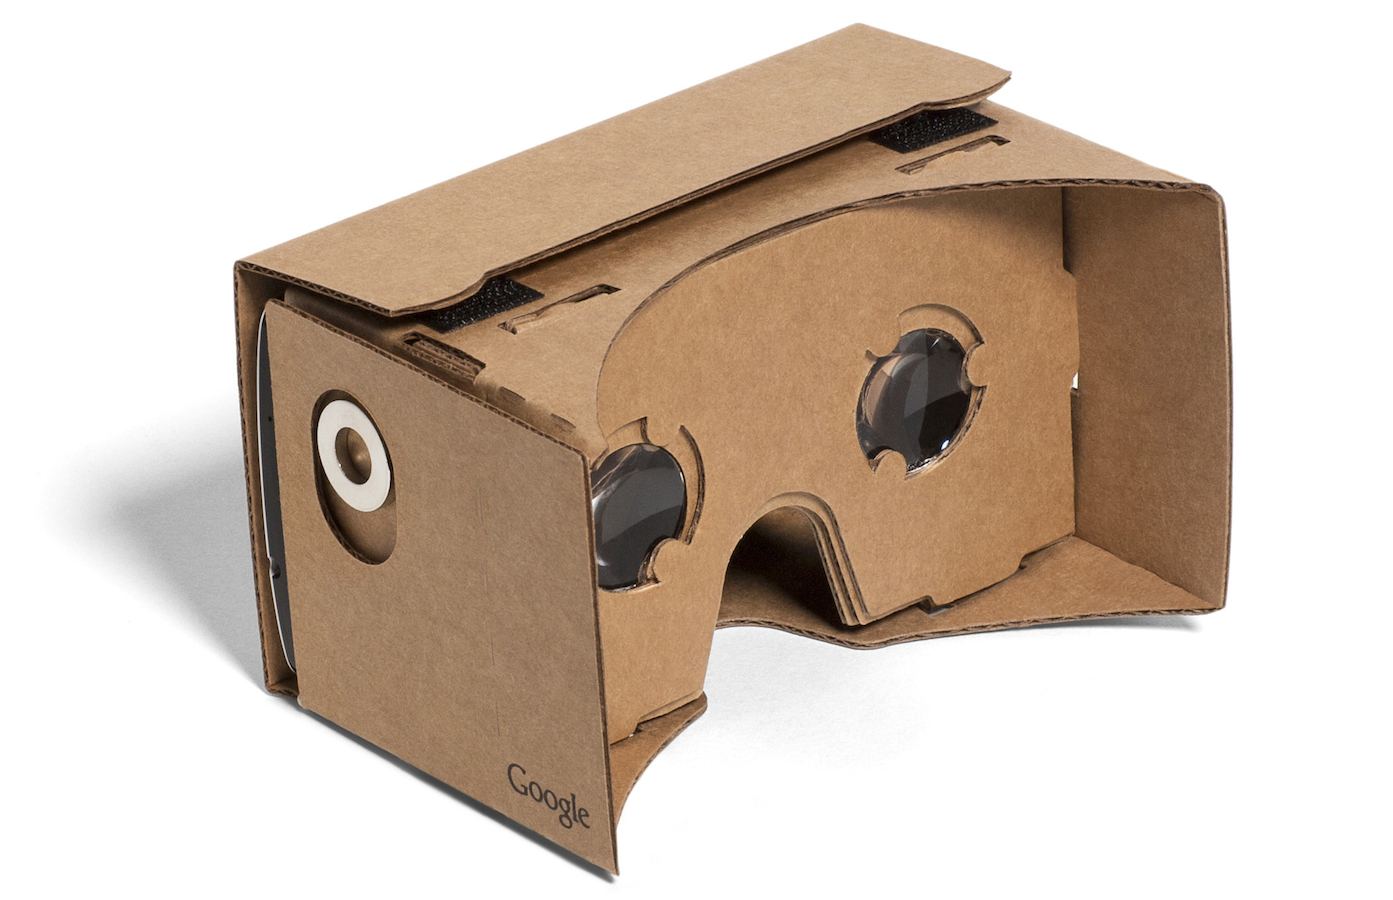
\includegraphics[scale=0.8]{cardboard}
		\hypertarget{gc}{\caption{Visore per la realtà virtuale \textit{Google Cardboard}}}
	\end{center}
\end{figure}
\FloatBarrier